%-*- coding:utf-8 -*-

\documentclass[10pt,dvipdfmx]{beamer}
\usepackage{tutorial}

\title{計算機実験II (L1) --- モンテカルロ法}
\date{2021/10/08}

\begin{document}

\begin{frame}
  \titlepage
  \tableofcontents
\end{frame}

\section{講義・実習の概要}

\begin{frame}[t]{講義・実習の目的}
  \begin{itemize}
    %\setlength{\itemsep}{1em}
  \item 理論・実験を問わず、学部〜大学院〜で必要となる現代的かつ普遍的な計算機の素養を身につける
  \item {\color{gray}UNIX環境に慣れる(シェル、ファイル操作、エディタ)}
  \item {\color{gray}ネットワークの活用 (リモートログイン、共同作業)}
  \item {\color{gray}プログラムの作成(C言語、コンパイラ、プログラム実行)}
  \item 基本的な数値計算アルゴリズム・数値計算の常識を学ぶ
  \item {\color{gray}科学技術文書作成に慣れる(\LaTeX, グラフ作成)}
  \item {\color{red}物理学における具体的な問題を通して実践的な知識と経験を身につける}
  \end{itemize}
\end{frame}

\begin{frame}[t]{身に付けて欲しいこと}
  \begin{itemize}
    %\setlength{\itemsep}{1em}
  \item ツールとしてないものは自分で作る (物理の伝統)
  \item すでにあるものは積極的に再利用する (車輪の再発明をしない)
  \item 数学公式と数値計算アルゴリズムは別物
  \item 刻み幅・近似度合いを変えて何度か計算を行う
  \item グラフ化して目で見てみる
  \item 計算量(コスト)のスケーリング(次数)に気をつける
  \item (計算機は指示したことを指示したようにしかやってくれないということを認識する)
  \item {\color{red}問題の解き方は一通りではない}
  \item {\color{red}いろいろな手法を組み合わせて使う}
  \end{itemize}
\end{frame}

\begin{frame}[t]{講義・実習内容}
  \begin{itemize}
    \setlength{\itemsep}{1em}
  \item 問題解決型: 計算機実験Iで身に付けた知識をもとに、より高度な数値計算手法・アルゴリズムを学び、物理学における具体的な問題への応用を通して実践的な知識と経験を身につける
    \begin{itemize}
    \item 取り上げる問題
      \begin{itemize}
      \item ランダムプロセス
      \item 統計力学(イジング模型)
      \item 拡散方程式、波動方程式
      \item 量子力学(1粒子系、実時間発展、横磁場イジング模型、量子コンピュータ)
      \item 力学系・粒子系
        
      \end{itemize}
    \item 取り上げる計算手法・アルゴリズム
      \begin{itemize}
      \item モンテカルロ法・マルコフ連鎖モンテカルロ法
      \item 行列の対角化・疎行列分解
      \item 有限差分法、偏微分方程式の解法
      \item 常微分方程式の積分、分子動力学
      \item 連続最適化、離散最適化
      \end{itemize}
    \end{itemize}
    などを予定
  \end{itemize}
\end{frame}

\begin{frame}[t]{講義日程 (予定)}
  \begin{itemize}
    % \setlength{\itemsep}{1em}
  \item 全8回 (金曜5限 16:50-18:35)
    \begin{itemize}
    \item 10月4日(金) 講義1: 多体系の統計力学とモンテカルロ法
    \item {\color{gray} 10月11日(金) 休講 (物理学教室コロキウム)}
    \item 10月18日(金) 実習1
    \item {\color{gray} 10月25日(金) 休講}
    \item 11月1日(金) 講義2: 偏微分方程式と多体系の量子力学
    \item 11月8日(金) 実習2
    \item {\color{gray} 11月15日(金) 休講}
    \item 11月29日(金) 講義3: 少数多体系・分子動力学
    \item 12月6日(金) 実習3
    \item {\color{gray} 12月13日(金) 休講 (物理学教室コロキウム)}
    \item {\color{gray} 12月20日(金) 休講 (ニュートン祭)}
    \item 12月27日(金) 講義4: 最適化問題
    \item 1月10日(金) 実習4
    \item {\color{gray} 1月24日(金) 休講 (物理学教室コロキウム)}
    \end{itemize}
  \end{itemize}
\end{frame}


\begin{frame}[t,fragile]{講義と実習}
  \begin{itemize}
    %\setlength{\itemsep}{1em}
  \item スタッフ \href{mailto:computer@phys.s.u-tokyo.ac.jp}{computer@phys.s.u-tokyo.ac.jp}
    \begin{itemize}
    \item 講義: 藤堂
    \item 実習: 山崎助教、石河助教
    \item 実習TA: 猪俣
    \end{itemize}
  \item 講義・実習の進め方
    \begin{itemize}
    \item 講義(座学)と実習を実施
    \item 実習の回には各自PCを持参すること
    \end{itemize}
  \item 評価
    \begin{itemize}
    \item 出席(UTOLでのアンケートに回答)

      講義・実習当日16:50-20:00の間に回答
      
    \item レポート (計2回)
    \end{itemize}    
  \end{itemize}    
\end{frame}

% \section{環境整備}

\begin{frame}[t,fragile]{計算機実験に必要な環境整備}
  \begin{itemize}
    % \setlength{\itemsep}{1em}
  \item 「\href{https://github.com/utphys-comp/handbook/releases/download/handbook-2021/handbook.pdf}{計算機実験ハンドブック}」に書いてあることが、自宅のPCでも一通り試せるような環境を準備する
    \begin{itemize}
      % \setlength{\itemsep}{1em}
    \item プログラミング (オフライン・リモート利用)

      エディタ、コンパイラ(C, C++, Fortran, BLAS/LAPACK, MPI/OpenMP)
    \item 計算結果のプロット (オフライン利用)

      gnuplot (python/matplotlib, MATLAB でも可)
    \item 文書(レポート、論文)の作成 (オフライン・クラウド利用)

      \LaTeX (TeX Live あるいは Overleaf)
    \item ネットワークの利用 (ECCSなどの大学の計算機にリモートアクセスできる環境)

      ターミナル、SSH
    \item インタプリタ環境 (オフライン・クラウド利用)

      MATLAB、Python 2/3
    \end{itemize}
  \item 「\href{https://utphys-comp.github.io}{計算機実験のための環境整備}」({\small \href{https://utphys-comp.github.io}{https://utphys-comp.github.io}})を参考に、各自必要な環境を整備する
  \end{itemize}
\end{frame}



\section{乱択アルゴリズム}
\begin{frame}[t,fragile]{乱択アルゴリズム(randomized algorithm)}
  \begin{itemize}
    \setlength{\itemsep}{1em}
  \item 実行中に乱数を参照してその値によって振る舞いをかえるアルゴリズム
  \item ラスベガスアルゴリズム
    \begin{itemize}
    \item 乱数の出方によらず常に正しい結果を与えるアルゴリズム
    \item 平均化効果を利用するアルゴリズム:クイックソート
    \end{itemize}
  \item モンテカルロアルゴリズム
    \begin{itemize}
    \item 乱数の出方によっては誤った結果を与えるアルゴリズム
    \item 標本を利用するアルゴリズム:最大カット問題
    \item くじ引き型のアルゴリズム:素数性判定、関数の同一性、行列積の検算
    \item サンプリングアルゴリズム:モンテカルロ積分、マルコフ連鎖モンテカルロ
    \end{itemize}
  \end{itemize}
\end{frame}

\begin{frame}[t,fragile]{乱択クイックソート}
  \begin{itemize}
    \setlength{\itemsep}{1em}
  \item 分割統治法に基づく再帰的なソートアルゴリズム
    \begin{itemize}
      \item 配列の中から要素を一つ選び、それより小さい要素からのみなる集合と大きい要素のみからなる集合の2つに分ける
      \item それぞれの集合をソートし、結合する
    \end{itemize}
    \item ほぼ同じ大きさの集合に分けることができる場合の実行ステップ数$\sim {\cal O}(n \log n)$
    \item 最悪(選んだ要素が常に最大 or 最小値)の場合のステップ数$\sim {\cal O}(n^2)$
    \item 分割に用いる要素を「ランダムに」選ぶ $\Rightarrow$ 平均ステップ数$\sim {\cal O}(n \log n)$
  \end{itemize}
\end{frame}

\begin{frame}[t,fragile]{クイックソート}
  \resizebox{!}{.7\textheight}{\includegraphics{image/quicksort.pdf}}
\end{frame}

%-*- coding:utf-8 -*-

\begin{frame}[t,fragile]{最小カット問題}
  \begin{itemize}
    %\setlength{\itemsep}{1em}
  \item 「最小カット (min-cut)」= 連結グラフを二つの部分に分けるために切らなければならない辺(エッジ)の集合のうち、もっとも小さいもの
  \item ``Randomized Min-Cut Algorithm''
    \begin{itemize}
    \item ランダムに辺を一つ選ぶ
    \item 辺の両端の頂点を一つにつぶす(自己ループは取り除く)
    \item 残りの頂点が二つになるまで繰り返す
    \end{itemize}
  \item 上の試行を何回も繰り返して、得られたうちで最小なカットを結果とする
  \item 頂点の数が $n$ のグラフに関して、正解が得られる確率:少なくとも $\frac{2}{n(n-1)}$
  \end{itemize}
\end{frame}

\begin{frame}[t,fragile]{最小カット問題}
  \resizebox{!}{.6\textheight}{\includegraphics{image/min-cut.pdf}}
\end{frame}


\section{物理過程のシミュレーション}
\begin{frame}[t,fragile]{物質中の中性子輸送}
  \begin{center}
  \resizebox{0.45\textwidth}{!}{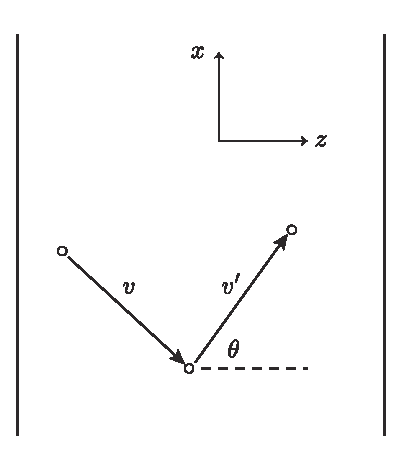
\includegraphics{image/scattering.pdf}}
  \end{center}
\end{frame}

\begin{frame}[t,fragile]{物質中の中性子輸送}
  \begin{itemize}
    %\setlength{\itemsep}{1em}
  \item ある板状の物質(厚さ$D$)に垂直に中性子が入射したときの吸収率・透過率・反射率
  \item 中性子はある確率で物質の原子核に衝突し、確率$p_{\rm c}$で吸収、$p_{\rm s}=1-p_{\rm c}$で散乱される
    \begin{itemize}
    \item 衝突は確率的に起きるので、次の衝突までの距離$\ell$は指数分布にしたがう($\lambda^{-1}$: 平均自由行程)
      \[
      p(\ell) = \lambda e^{-\lambda\ell}
      \]
    \item 衝突時、ランダムな方向に散乱されるとすると
      \[
      p(\theta,\phi) \, d\theta \, d\phi = \frac{d\Omega}{4\pi} = \frac{\sin \theta}{4\pi} \, d\theta \, d\phi
      \]
      \[
      p(\theta) = \frac{\sin \theta}{2} \qquad p(\phi)=\frac{1}{2\pi}
      \]
    \end{itemize}
  \end{itemize}
\end{frame}

\begin{frame}[t,fragile]{モンテカルロシミュレーション}
  \begin{enumerate}
    %\setlength{\itemsep}{1em}
  \item 初期条件 $z=0$, $\theta = 0$
  \item {\color{red} 指数分布から$\ell$を選ぶ}
  \item $z \leftarrow z + \ell \cos \theta$
  \item $z<0$ → 反射(終了) \\
    $z>D$ → 透過(終了) \\
    $0 < z < D$ → 確率$p_{\rm c}$で吸収(終了)、$p_{\rm s}$で散乱
  \item {\color{red} 散乱後の$\theta$を選び}、2に戻る
  \end{enumerate}
  \vspace*{-3.5cm}\hspace{8cm}\resizebox{0.25\textwidth}{!}{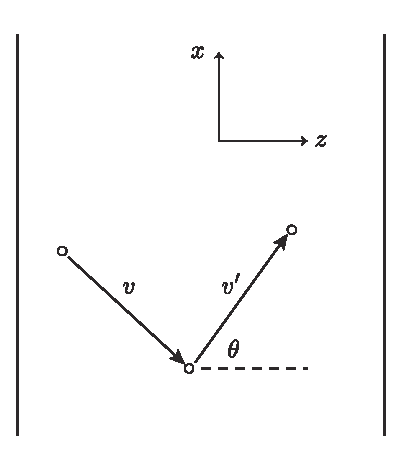
\includegraphics{image/scattering.pdf}}
\end{frame}


\section{擬似乱数}
\begin{frame}[t,fragile]{乱数}
  \begin{itemize}
    %\setlength{\itemsep}{1em}
  \item 自然乱数 (ハードウェア乱数)
    \begin{itemize}
    \item さいころ、コイン、ルーレット、核分裂反応、熱雑音、ショット雑音 ...
    \end{itemize}
  \item 疑似乱数とは
    \begin{itemize}
    \item 計算機でプログラムに従って生成する乱数(のようなもの)
    \item 乱数は何に役立つか?
      \begin{itemize}
      \item 等式のチェック、例外の発見
      \item 初期値にランダムネスを入れることで最悪の場合を避ける
      \item サンプリングを使ったシミュレーション (→計算機実験II)
      \end{itemize}
    \item 疑似乱数に必要な条件
      \begin{itemize}
      \item 多数の乱数が生成可能
      \item ポータビリティ
      \item 生成速度
      \item 再現性
      \item 統計的性質
      \end{itemize}
  %% \item 擬似乱数 (pseudo random number)
  %%   \begin{itemize}
  %%   \item 計算機でプログラムに従って生成
  %%   \item 分布の一様性、相関、周期に注意する必要あり
    \end{itemize}
  \end{itemize}
\end{frame}

\begin{frame}[t,fragile]{擬似乱数発生器の例}
  \begin{itemize}
    %\setlength{\itemsep}{1em}
  \item 最も簡単な乱数発生器:線形合同法 (linear congruential method)
    \[
    x_{n+1} = (ax_n+c) \ \mbox{mod} \ m
    \]
  \item 例) $a = 65539$, $c = 0$, $m = 2147483648$ (周期 $m-1$)
  \item 少しだけ異なる初期値 $(x0 = 1, 2, 3)$ から始めた場合
  \resizebox{!}{.35\textheight}{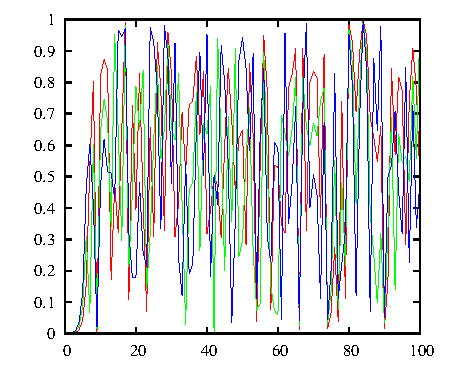
\includegraphics{image/lcg-1.pdf}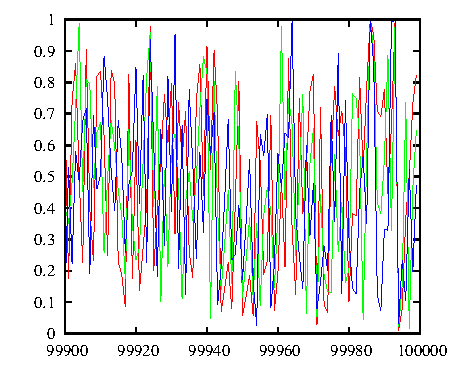
\includegraphics{image/lcg-2.pdf}}
  \item 数十ステップ進むとバラバラな振舞い ⇒ カオス的?
  \end{itemize}
\end{frame}

\begin{frame}[t,fragile]{擬似乱数生成器における相関}
  \begin{itemize}
    %\setlength{\itemsep}{1em}
  \item 合同乗算法で多次元超立方体中に「ランダムに」点を打つと、それらの点は全て比較的小数の等間隔に並んだ超平面の上にのってしまう (多次元疎結晶構造)

    \resizebox{!}{.35\textheight}{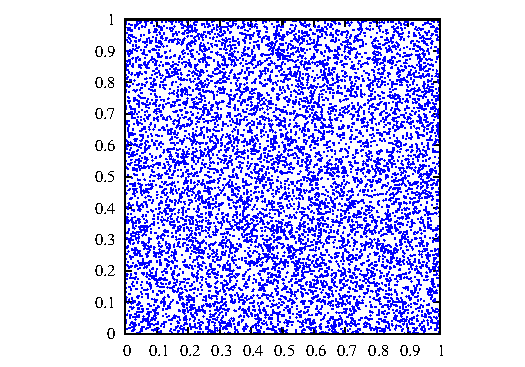
\includegraphics{image/lcg-2d.pdf}}
    \resizebox{!}{.35\textheight}{\includegraphics{image/lcg-3d.pdf}}
    
  \item 計算式に従って生成するため、必ず何らかの相関は残る
  \item できる限り相関が少なく周期の長い、理想的な乱数の開発が続けられている
    \begin{itemize}
    \item 現時点で、標準的な乱数発生器:メルセンヌ・ツイスター
    \item 周期 $2^{19937}-1$、高速、日本製! (例: \href{https://github.com/todo-group/computer-experiments/blob/master/exercise/monte_carlo/random.c}{random.c})
    \end{itemize}
  \end{itemize}
\end{frame}

\begin{frame}[t,fragile]{乱数発生器の選び方}
  \begin{itemize}
    %\setlength{\itemsep}{1em}
  \item 疑似乱数を使う場合の注意
    \begin{itemize}
    \item 万能乱数発生器は存在しない
    \item 計算式に従って生成するため、必ず周期は有限、何らかの相関あり
    \item 乱数の性質について、数学的に厳密な証明やテスト結果があるが、特定のシミュレーションに使う場合について何も保証してくれない
    \item 自分で乱数発生器を「発明」してはいけない
    \item 自分で乱数発生器をプログラムしてはいけない(既存のライブラリを使う)
    \item 初期化(種・シードの設定)を正しく行う
    \item 実際にそれらしい乱数が生成されているか、グラフに描いて確認する
    \item 二種類以上の乱数発生器を使ってみて、結果が一致するか確認
    \end{itemize}
  \item 代表的な乱数発生器のひとつ: メルセンヌ・ツイスター
    \begin{itemize}
    \item 周期 $2^{19937}-1$、高速、日本製!
    \item ヘッダファイル: \href{https://github.com/todo-group/computer-experiments/blob/master/exercise/monte_carlo/mersenne_twister.h}{mersenne\_twister.h}
    \item サンプルプログラム: \href{https://github.com/todo-group/computer-experiments/blob/master/exercise/monte_carlo/random.c}{random.c}
    \end{itemize}
  \end{itemize}
\end{frame}

\begin{frame}[t,fragile]{様々な分布}
  \begin{itemize}
    %\setlength{\itemsep}{1em}
  \item 乱数発生器は通常、一様な整数乱数あるいは実数乱数を生成
  \item 一様分布以外の分布にしたがう乱数の発生方法の代表例
  \item 逆関数法
    \begin{itemize}
      \item 確率分布関数$F(x)$の逆関数$F^{-1}(y)$ と(0,1)の一様乱数$u$から $v=F^{-1}(u)$
      \item 例: 指数分布 $p(x) = \frac{1}{\mu} e^{-x/\mu}$

      $F(x) = 1 - e^{-x/\mu}$ \ \ \ $F^{-1}(y) = - \mu \log(1-y)$
      \item 一般の確率分布関数について逆関数を求めるのは困難
    \end{itemize}
  \item 棄却法
    \begin{itemize}
      \item 確率密度関数を完全に囲むような箱を用意し、その箱の中で一様乱数を生成
      \item 確率密度関数の下側の点が生成されたら、その$x$座標を乱数として採用。上側の点の場合には再度生成
      \item もとの確率密度関数よりも箱が大きくなりすぎると非効率
    \end{itemize}
  \end{itemize}
\end{frame}

%-*- coding:utf-8 -*-

\begin{frame}[t,fragile]{Box-Muller法}
  \begin{itemize}
    %\setlength{\itemsep}{1em}
  \item 一様分布乱数から正規分布乱数を生成する方法
    \begin{itemize}
    \item 2次元の(標準)ガウス分布を考える
      \[
      f(x,y)\,dx\,dy= \frac{1}{2\pi} e^{-(x^2+y^2)/2} \,dx\,dy
      \]
    \item 極座標$(r,\theta)$に変換 ($x=r\cos\theta$, $y=r\sin\theta$)
      \[
      \frac{1}{2\pi} e^{-(x^2+y^2)/2} \,dx\,dy = \frac{1}{2\pi} r \, e^{-r^2/2} \,dr\,d\theta
      \]
    \item $\theta$は$(0,2\pi)$の一様分布
    \item $r$は$f(r) = r \, e^{-r^2/2}$に従う
      \begin{align*}
        F(r) = \int_0^r f(r) \, dr = 1 - e^{-r^2/2}, \qquad r = F^{-1}(q) = \sqrt{- 2 \log(1-q)}
      \end{align*}
    \item 二つの一様乱数から二つの独立な正規分布乱数が生成される
    \end{itemize}
  \end{itemize}
\end{frame}


%-*- coding:utf-8 -*-

\section{ヒストグラム}

\begin{frame}[t,fragile]{ヒストグラムの作り方}
  \begin{itemize}
    %\setlength{\itemsep}{1em}
  \item 連続変数(実数)のデータの場合 ([]内はサンプルプログラムでの変数名)
    \begin{itemize}
    \item $N$: サンプル数 [{\tt samples}]
    \item $x_{\rm min}$: データの最小値(カットオフ) [{\tt xmin}]
    \item $x_{\rm max}$: データの最大値(カットオフ) [{\tt xmax}]
    \item $n$: ビンの個数 [{\tt bins}]
    \item $\Delta$: ビンの幅 ($\Delta=(x_{\rm max}-x_{\rm min}) / n$) [{\tt dx}]
    \end{itemize}
  \item サイズ$n$の配列を準備
    \begin{itemize}
    \item データ毎にどのビンに入るか計算: $j = (x - x_{\rm min}) / \Delta$
    \item (必要に応じて) $0 \le j < n$であることを確認 (範囲外のデータは無視する)
    \item 配列の$j$番目の値を1増やす
    \end{itemize}
    \item サンプルプログラム: \href{https://github.com/todo-group/computer-experiments/blob/master/exercise/monte_carlo/histogram.c}{histogram.c}
  \end{itemize}
  \vspace*{-5cm} \hfill \resizebox{0.28\textwidth}{!}{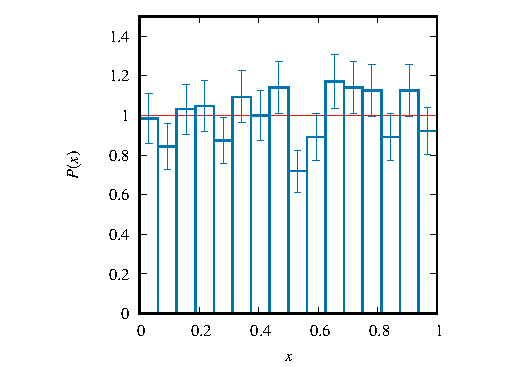
\includegraphics{image/histogram.pdf}}
\end{frame}

\begin{frame}[t,fragile]{ビンの個数の設定}
  \begin{itemize}
  \item 最適の幅というものはない
  \item 個数を増やすと表現の自由度は増えるが、各ビンのエラーバーが大きくなる
    \begin{itemize}
    \item データが統計的に独立である場合、それぞれのビンのカウント数$m$はポワソン分布に従う
    \item 統計誤差 $\sim \sqrt{m}$
    \end{itemize}
  \item いくつかの方法・公式が提案されているが、分布の形によっては不適切な場合も
    \begin{itemize}
    \item スタージェスの公式 $n = \log_2 N + 1$
    \item スコットの公式 $\Delta = 3.5 \sigma / N^{1/3}$
    \end{itemize}
  \item 実際には、ビンの個数を何通りか試してみるのが良い
  \item データを取り直すことが出来ない and/or コストがかかる場合も多いので、生データはいったんファイルに保存しておく
  \end{itemize}
\end{frame}


%-*- coding:utf-8 -*-

\section{モンテカルロ積分}

\begin{frame}[t,fragile]{モンテカルロ積分}
  \begin{itemize}
    \setlength{\itemsep}{1em}
  \item 円周率を与える公式
    \[
    \pi = \lim_{c \rightarrow \infty} \int_0^c f(x) \, dx \ \ \ f(x) = \frac{2}{\cosh x}
    \]
  \item スタンダードな数値積分法: 台形公式 (一次式補間), シンプソン公式 (二次式補間), etc
  \item カットオフ $c$ の値
    \begin{itemize}
    \item 誤差は $c$ が大きくなると指数関数的に小さくなる
    \item 例えば $c = 20$ で誤差は $8.3 \times 10^{-9}$ 以下
    \end{itemize}
  \end{itemize}
\end{frame}

\begin{frame}[t,fragile]{単純サンプリング}
  \begin{itemize}
    \setlength{\itemsep}{1em}
  \item $[0,c]$ と $[0,2]$ の一様分布から二次元上の点 $(x,y)$ を $M$ 組生成
  \item $f(x)$ の下に入った数 $N$ をカウント
    \[
    \pi \simeq 2c \times \frac{N}{M}
    \]
    \begin{tabular}{|c|c|c|}
      \hline
      $M$ & 平均値 & 誤差 \\
      \hline
      100 & 4.8 & 1.3 \\
      10000 & 3.12 & 0.11 \\
      1000000 & 3.154 & 0.011 \\
      \hline
    \end{tabular}
  \end{itemize}
  \vspace*{-7em}
  \hspace*{17em}
  \resizebox{!}{.45\textheight}{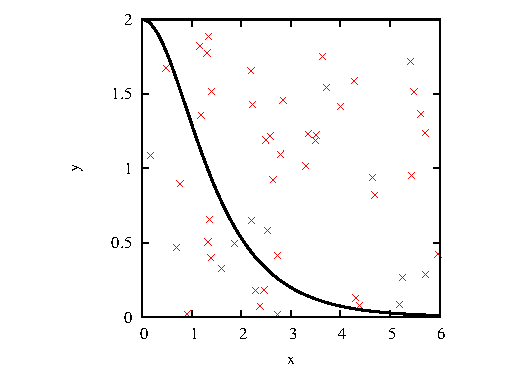
\includegraphics{image/coth-1.pdf}}
\end{frame}

\begin{frame}[t,fragile]{統計誤差の評価}
  \begin{itemize}
    \setlength{\itemsep}{1em}
  \item このモンテカルロ積分が実際に評価している積分
    \[
    \frac{1}{2c} \int_0^c \!\! \int_0^2 \!\! \theta(x,y) \, dx \, dy
    \ \ \ \theta(x,y) = \begin{cases} 2c & \text{if $y < f(x)$} \\ 0 & \text{otherwise} \end{cases}
    \]
  \item 統計誤差の評価
    \begin{itemize}
      \item 試行の成功確率(success probability): $q=\frac{\pi}{2c}$
      \item 一回の試行の平均値(mean): $\mu = 2c \times q = \pi$
      \item 分散(variance):
        \[ s^2 = (2c)^2q + 0^2(1-q) - \mu^2 = 2c\pi-\pi^2 = 4c^2 q(1-q) \]
      \item $c=20$ の時:
        \[ q \simeq 0.0785 \ \ \ s^2 \simeq 116
        \]
    \end{itemize}
  \end{itemize}
\end{frame}

\begin{frame}[t,fragile]{中心極限定理(central limiting theorem)}
  \begin{itemize}
    %\setlength{\itemsep}{1em}
  \item $M$回の試行のうち $N$回成功する確率 ($\pi$の見積もり値が $m=2cN/M$ となる確率)
    \[
    p(m=2c\frac{N}{M}) = \frac{M!}{N!(M-N)!} q^N (1-q)^{M-N}
    \]
  \item 両辺の対数をとってスターリングの公式を使う
    \[
    \log p(m) \simeq \frac{M}{2c} (m \log \frac{\pi}{m} + (2c-m)\log \frac{2c-\pi}{2c-m})
    \]
  \item $m$ に関して平均値 $\pi$ の周りで二次まで展開
    \[
    \log p(m) \simeq -\frac{M}{2s^2}(m-\pi)^2
    \]
  \item 分散$s^2/M$の正規分布(中心極限定理)
  \item 統計誤差は $\sqrt{M}$ に反比例して減少 $\Rightarrow$ 1桁小さくするには100倍の計算が必要
  \end{itemize}
\end{frame}

\begin{frame}[t,fragile]{単純サンプリング(2)}
  \begin{itemize}
    \setlength{\itemsep}{1em}
  \item $y$ に関してあらかじめ積分
  \item $[0,c]$の一様乱数 $x$ を用いて
    \[
    \int_0^c \frac{f(x)}{p(x)} p(x) \, dx \simeq \frac{1}{M} \sum_i c f(x_i) \ \ \ p(x) = \frac{1}{c}
    \]
    \begin{tabular}{|c|c|c|}
      \hline
      $M$ & 平均値 & 誤差 \\
      \hline
      100 & 3.1 & 0.8 \\
      10000 & 3.00 & 0.08 \\
      1000000 & 3.147 & 0.008 \\
      \hline
    \end{tabular}
  \end{itemize}
  \vspace*{-7em}
  \hspace*{17em}
  \resizebox{!}{.45\textheight}{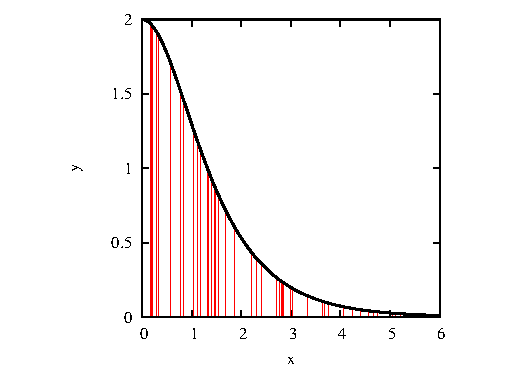
\includegraphics{image/coth-2.pdf}}
\end{frame}

\begin{frame}[t,fragile]{誤差の評価}
  \begin{itemize}
    \setlength{\itemsep}{1em}
  \item 関数 $f(x)/p(x)$ の分散
    \[
    s^2 = \int_0^c \Big(\frac{f(x)}{p(x)}\Big)^2 p(x) \, dx - \pi^2 = c \int_0^\infty f^2(x) \, dx - \pi^2 = 4c - \pi^2
    \]
  \item $c=20$ のとき $s^2 \simeq 70.1$
  \item 同じ試行回数 $M$ の時, 誤差は$\sqrt{70.1/116} = 0.77$ 倍
  \item もしくは $M$ を $116/70.1 = 1.65$ 倍したのと同じ効果
  \item 積分次元は低ければ低いほど良い
  \end{itemize}
\end{frame}

\begin{frame}[t,fragile]{次元の呪い(curse of dimensionality)}
  \begin{itemize}
    %\setlength{\itemsep}{1em}
  \item $n$次元超立方体(1辺の長さ 2, 体積 $2^n$)に対する$n$次元単位球の体積の割合
    \[
    q = \frac{\pi^{n/2} / \Gamma(\frac{n}{2}+1)}{2^n} \sim (\pi/n)^{n/2}
    \]
    $n=10$ で 0.2\%, $n=20$ で $10^{-8}$, $n=100$ で $10^{-70}$
  \item モンテカルロ積分で球の体積を計算しようとすると, 標準偏差に対する平均値の割合は指数関数的に小さい
    \[
    \frac{q}{\sqrt{q(1-q)}} \sim \sqrt{q}
    \]
  \item 次元が高くなるにつれて指数関数的に大きな $M$ が必要となる
  \item c.f. 通常の数値積分(台形公式等)でも同様
  \end{itemize}
\end{frame}

\begin{frame}[t,fragile]{重点的サンプリング}
  \begin{itemize}
    \setlength{\itemsep}{1em}
  \item (平均値が同じなら)被積分関数の分散が小さければ小さいほど良い (= 統計誤差が小さい)
  \item サンプリングの分布 $p(x)$ の形が $f(x)$ に近い程良い
  \item $f(x)$ の値が大きい所はより頻繁にサンプリング
  \item 重点的サンプリング (importance sampling)
  \end{itemize}
\end{frame}

\begin{frame}[t,fragile]{重点的サンプリング}
  \begin{itemize}
    \setlength{\itemsep}{1em}
  \item 積分への寄与が大きな箇所をより重点的にサンプリング
    \[
    p(x) = e^{-x}
    \]
    \begin{tabular}{|c|c|c|}
      \hline
      $M$ & 平均値 & 誤差 \\
      \hline
      100 & 3.06 & 0.06 \\
      10000 & 3.142 & 0.006 \\
      1000000 & 3.1412 & 0.0006 \\
      \hline
    \end{tabular}
  \end{itemize}
  \vspace*{-7em}
  \hspace*{17em}
  \resizebox{!}{.45\textheight}{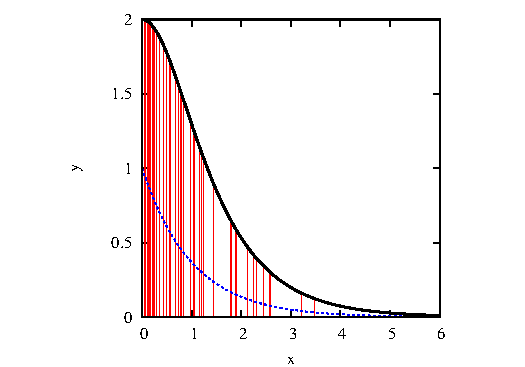
\includegraphics{image/coth-3.pdf}}
\end{frame}

\begin{frame}[t,fragile]{誤差のサンプル数依存性}
  \begin{itemize}
    \setlength{\itemsep}{1em}
  \item 関数 $f(x)/p(x)$ の分散
    \[
    s^2 = \int_0^c \Big(\frac{f(x)}{p(x)}\Big)^2 p(x) \, dx - \pi^2 \simeq 2(2+\pi) - \pi^2 = 0.414
    \]
  \item 同じ試行回数 $M$ の時, 誤差は

    $\sqrt{0.414/116} = 0.06 \mbox{倍}$

  \item もしくは $M$ を 280 倍したのと同じ
  \vspace*{-5em}
  \hspace*{15em}
  \resizebox{!}{.45\textheight}{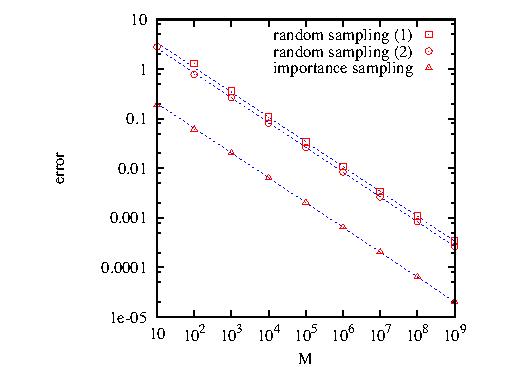
\includegraphics{image/sech-error.pdf}}
  \end{itemize}
\end{frame}

\begin{frame}[t,fragile]{理想的な重点的サンプリング?}
  \begin{itemize}
    \setlength{\itemsep}{1em}
  \item 理想的には $p(x)$ を $f(x)$ に比例するように取れば良い
  \item このとき $f(x) / p(x)$ は定数(分散 0) → 1回のサンプリングで厳密な結果が得られる???
  \item 実際には $p(x)$ が確率密度となるように規格化条件から定数 $c$ を決めておく必要あり
    \[
    \int p(x) \, dx = c \int f(x) \, dx = 1
    \]
  \item $c$ は今欲しい答そのもの!
  \end{itemize}
\end{frame}



\begin{frame}[t]{本日の課題}
  \begin{itemize}
    %\setlength{\itemsep}{1em}
  \item 「\href{https://utphys-comp.github.io}{計算機実験のための環境整備}」({\small \href{https://utphys-comp.github.io}{https://utphys-comp.github.io}})の確認
  \item 実習
    \begin{itemize}
    \item 講義資料の中の {\tt random.c}, {\tt histogram.c}をコンパイル・実行。ソースコードの中身を確認 \\
      サンプルコード一式: \href{https://github.com/todo-group/ComputerExperiments/releases/tag/2021a-computer2}{example-2.zip}
    \item ヒストグラムのプロットをしてみる
    \item 実習課題一覧\href{https://github.com/todo-group/ComputerExperiments/releases/tag/2021a-computer2}{exercise-2.pdf}の課題に取り組む
    \end{itemize}
  \item 質問はSlackの「\# 7\_モンテカルロ法」あるいは他の適当と思われるチャンネルで
  \item 本日24時までにITC-LMSのアンケート「第1回(10/08)作業レポート」に回答(出席のかわり)
  \end{itemize}
\end{frame}

\end{document}
